\documentclass[../mathNotesPreamble]{subfiles}
\begin{document}
%  \relscale{1.4}
  \section{8.4: Trigonometric Substitutions}

  \begin{ex*}
    Verify the formula for the area of a circle with radius $a$ by finding the area under $f(x)=\sqrt{a^2-x^2}$.
  \end{ex*}
  \begin{flushright}
    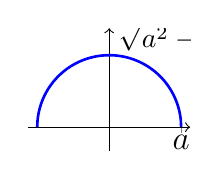
\begin{tikzpicture}
      \begin{axis}[
        axis lines=center,
        axis equal,
        axis line style={black,->},
        xmin=-4.5, xmax=4.5,
        ymin=-0.0625, ymax=4.25,
        xtick={4},
        xticklabels={$a$},
        ymajorticks=false,
        ticklabel style={font=\large,inner sep=0.5pt,fill=white,opacity=1.0, text opacity=1},
        every axis plot/.append style={line width=0.95pt, color=blue, samples=500}, 
        width=0.3\linewidth
        ]
        \addplot[-] expression[domain=-4:4]{sqrt(16-x^2)} node[pos=0.525, above right, black, font=\normalsize, inner sep=1pt] {$\sqrt{a^2-x^2}$};
      \end{axis}
    \end{tikzpicture}
  \end{flushright}
  \vspace*{\stretch{1}}

  \begin{center}
    \newcommand{\blankTriangle}[3]{
      \begin{tikzpicture}[scale=0.85]
        \coordinate (O) at (0,0);
        \coordinate (A) at (4,0);
        \coordinate (B) at (4,3);

        \tkzFillAngle[fill= ClemsonOrange!90,size=7.5mm, opacity=0.7](A,O,B);
        \tkzLabelAngle[pos = 1.1,font=\large](A,O,B){\color{black}$\theta$};
        \draw (O) -- node[below] {$#1$} (A) -- node[right] {$#2$} (B) -- node[above left] {$#3$} cycle;
      \end{tikzpicture}
    }
    \blankTriangle{\sqrt{a^2-u^2}}{u}{a} \hspace*{\stretch{1}}
    \blankTriangle{u}{a}{\sqrt{a^2-u^2}} \hspace*{\stretch{1}}
    \blankTriangle{a}{\sqrt{a^2-u^2}}{u}

    \addtolength{\jot}{15pt}
    \begin{alignat*}{4}\toprule
      &a^2-u^2 \hspace*{12mm}& 
      u&=a\sin(\theta),\hspace*{5mm}&
      &-\frac{\pi}{2}\leq \theta\leq \frac{\pi}{2}, \hspace*{2mm} \textnormal{ for } \abs{u}\leq a
       & \hspace*{12mm} a^2+a^2\sin^2(\theta)&=a^2\cos^2(\theta)\\
      %
      &a^2+u^2 &
      u&=a\tan(\theta),&
      &-\frac{\pi}{2}< \theta< \frac{\pi}{2},
       & a^2-a^2\tan^2(\theta)&=a^2\sec^2(\theta)\\
      %
      &u^2-a^2& 
      u&=a\sec(\theta),\ 
      &&\begin{cases}
        0\leq \theta< \frac{\pi}{2}, & \textnormal{ for } u\geq a\\
        \frac{\pi}{2}< \theta\leq \pi, & \textnormal{ for } u\leq -a
      \end{cases}
       & a^2\sec^2(\theta)-a^2&=a^2\tan^2(\theta)\\\bottomrule
    \end{alignat*}
  \end{center}
  \pagebreak

  \begin{ex*}
    $\displaystyle\int \frac{\sqrt{x^2-4}}{x^3}\,dx$
  \end{ex*}
  \vspace*{\stretch{1}}
  \pagebreak

  \begin{ex*}
    $\displaystyle\int \frac{\sqrt{16-x^2}}{x}\,dx$
  \end{ex*}
  \vspace*{\stretch{1}}
  \pagebreak

  \begin{ex*}
    $\displaystyle \int \frac{x^3}{\parens{25-4x^2}^{\nicefrac{3}{2}}}\,dx$
  \end{ex*}
  \vspace*{\stretch{1}}
  \pagebreak

  \begin{ex*}
    $\displaystyle \int_{0}^{\nicefrac{1}{3}} \frac{dx}{\parens{9x^2+1}^{\nicefrac{3}{2}}}$
  \end{ex*}
  \vspace*{\stretch{1}}
  \pagebreak

  \begin{ex*}
    $\displaystyle \int \frac{x}{\sqrt{x^2-2x+10}}$
  \end{ex*}
  \vspace*{\stretch{1}}
  \pagebreak

  \pagebreak

\end{document}
